% !TEX root = ../../main.tex
% !TeX spellcheck = de_DE

\chapter{Diskussion}
Ziel der Studienarbeit ist es, möglichst gute Architekturen inklusive Hyperparameterkombinationen zu finden.
Dafür werden in diesem Kapitel die Trainingsergebnisse des Dense-, und DC-GANs verglichen und interpretiert.

\section{Zusammenfassung der Ergebnisse}
\subsubsection{Dense GAN}
Die besten Ergebnisse erzielt das Dense GAN, das ausschließlich aus Dense Layern besteht.
Es ist in der Lage Figuren zu erzeugen, die Eigenschaften der Zielfiguren enthalten.
Außerdem sind die generierten Figuren stark abhängig vom jeweiligen Label.

Bei der Auswahl der Ergebnisse ist außerdem aufgefallen, dass die besten FID-Werte nicht mit den subjektiv besten Ergebnissen übereinstimmen.
\newline

Nach einem zusätzlichen Training der Hyperparameterkombination mit den subjektiv besten Ergebnissen sind die Figuren nochmals deutlich klarer abgebildet.
Allerdings hat das Dense GAN immer starke Schwierigkeiten mit Rauschen.
So sind zum einen immer Pixelfragmente im Bild zu erkennen oder die Figuren besitzen keine klaren Ränder.

\begin{figure}[H]
	\centering
	\subfloat[][]{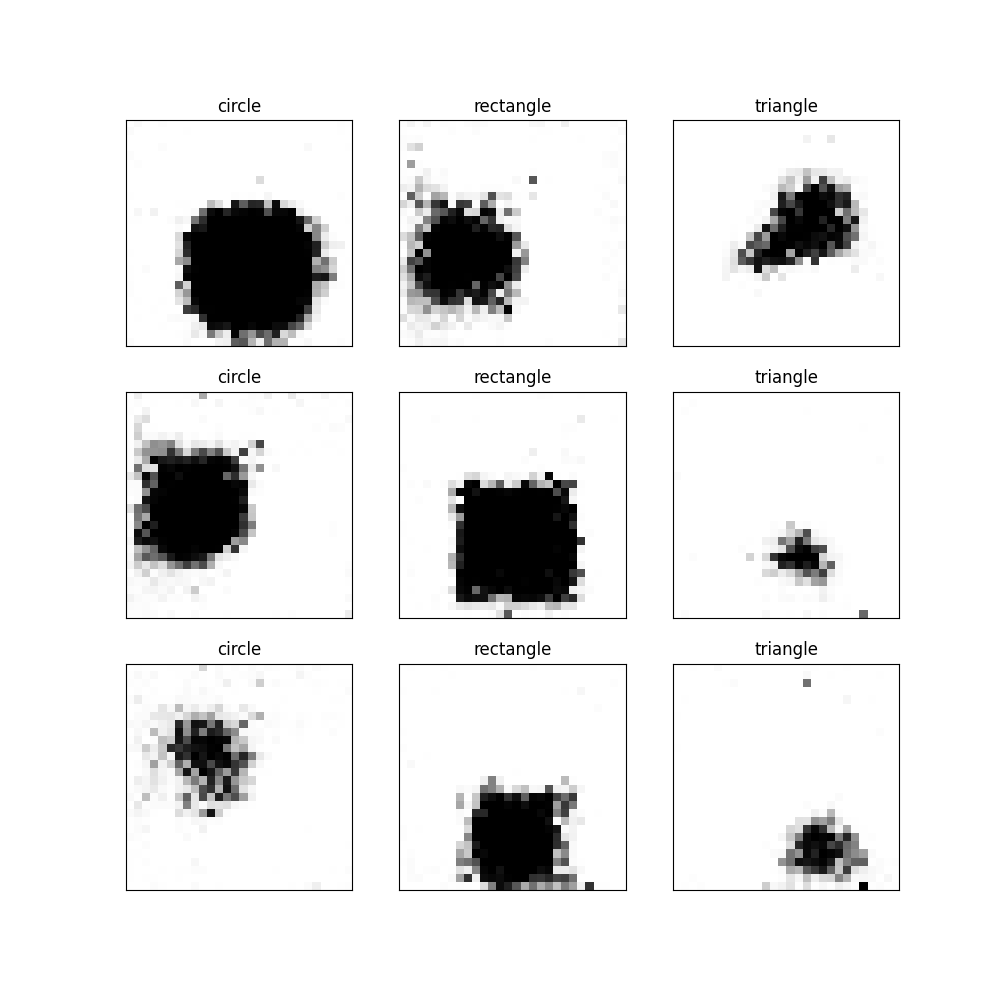
\includegraphics[width=0.45\linewidth]{kapitel/5_ergebnisse/densegan/good_example.png}}
	\qquad
	\subfloat[][]{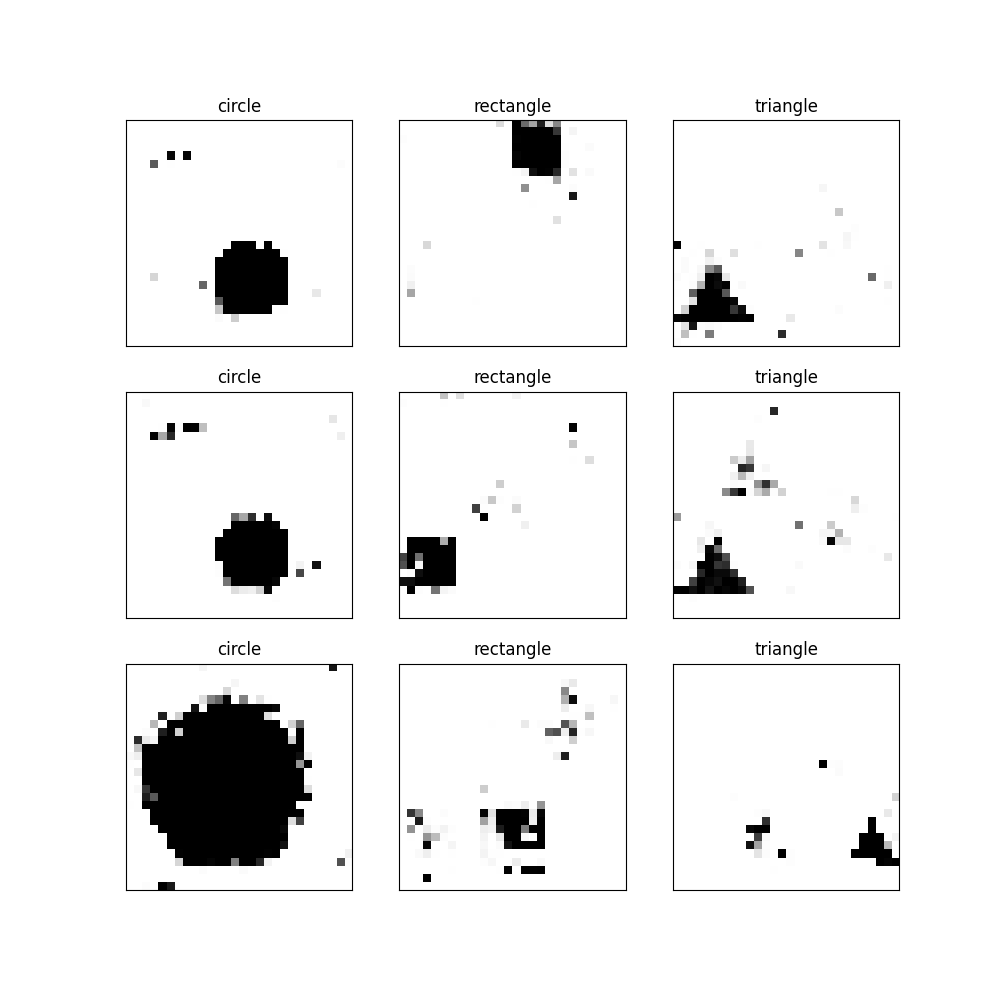
\includegraphics[height=0.35\textheight]{kapitel/5_ergebnisse/densegan/good_example_long.png}}
	\label{ergebnis:densegan-zusammenfassung}
	\caption[]{\textbf{a)} die subjektiv besten Ergebnisse nach regulärem Training; \textbf{b)} Ergebnisse nach zusätzlichem Training; \\auf beiden Bildern lässt sich starkes Rauschen erkennen}
\end{figure}

\subsubsection{DC GAN}
Probleme mit Rauschen existieren beim DC-GAN fast gar nicht, die Figuren sind alle sehr klar abgebildet.
Es existieren auch vergleichsweise wenig zusätzliche Pixelfragmente.
Die existierenden Pixelfragmente sind eher vergleichbar mit einer zweiten Figur auf dem Bild, da sie in Größe und Merkmalen nicht von der eigentlichen Figur zu unterscheiden sind.
Entsprechende Beispiele sind im \cref{ergebnis:dcgan-fid-zusammenfassung} zu sehen.
\newline

Allerdings ist die Qualität der DC-GAN-Bilder deutlich schlechter.
Oftmals wird eine Figur erzeugt, die Merkmale mehrere Kategorien besitzt.
Dabei handelt es sich zum Beispiel um einen Kreis mit einer geraden Kante oder Ecke.
Durch die Verschmelzung von Eigenschaften lassen sich die Figuren nicht immer eindeutig den geometrischen Formen zuordnen.

\begin{figure}[H]
	\centering
	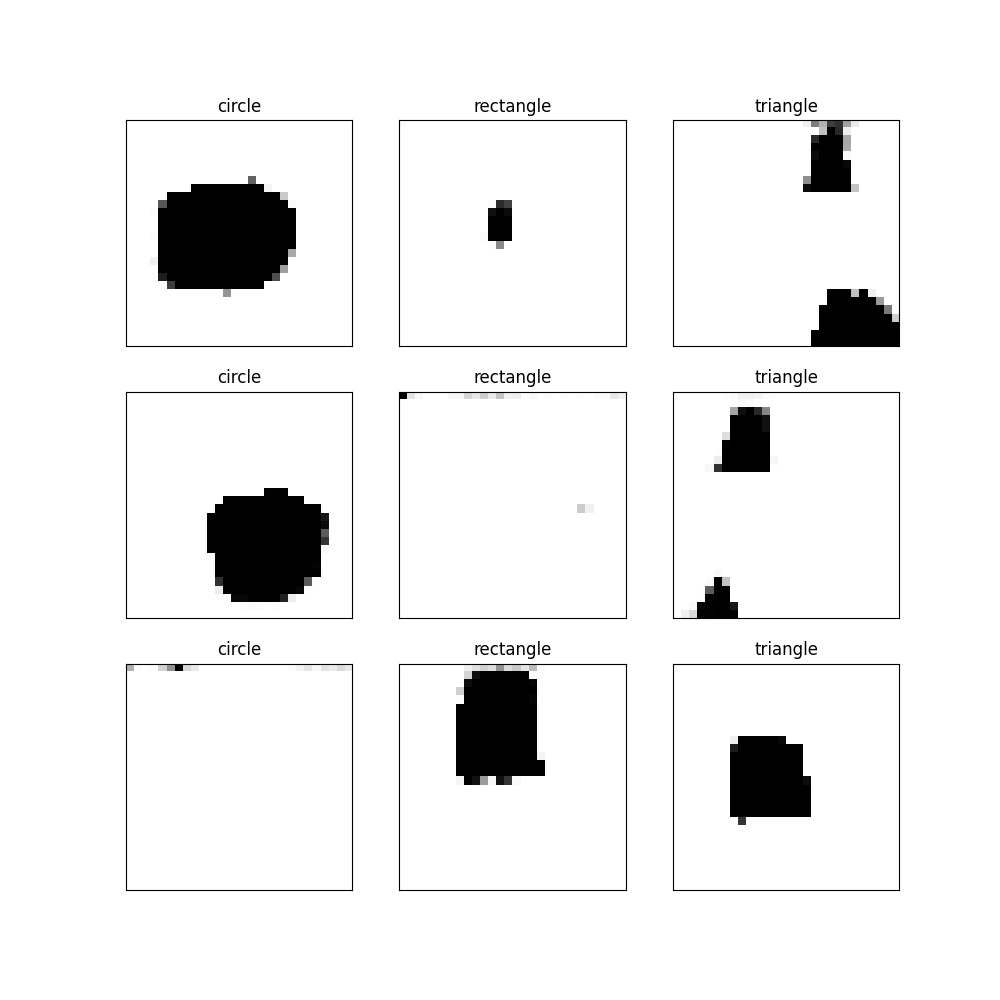
\includegraphics[width=0.45\linewidth]{kapitel/5_ergebnisse/dcgan/fid_circle.png}
	\label{ergebnis:dcgan-fid-zusammenfassung}
	\caption[]{\textbf{Oben Links:} ein Kreis mit einer geraden Kante; \textbf{Mitte Rechts:} zwei Pixelfragmente mit den schrägen Kanten eines Dreiecks}
\end{figure}

\subsubsection{Vergleich}
Insgesamt sind die Bilder des Dense GANs leicht besser als die Bilder des DC GANs.
Zwar sind sie deutlich verrauschter, aber die Figuren entsprechen mehr dem zugehörigen Label.
Beide Architekturen generieren jedoch keine Bilder, die von Menschen mit den Trainingsdaten verwechselt werden könnten.


\section{Interpretation der Ergebnisse}
Beide Architekturen erzeugen Bilder, die Gemeinsamkeiten mit den Trainingsdaten aufzeigen.
Unterschiede gibt es vor allem beim Rauschen und der Unterscheidbarkeit der Figuren.

\subsubsection{Rauschen}
Das Dense-GAN hat größere Probleme mit Rauschen.
Das lässt sich auf die Layerarchitektur zurück führen, da im Gegensatz zu Convolutional Layern die Pixel separater betrachtet werden.
Dadurch werden Zusammenhänge zwischen benachbarten Pixeln werden nicht so stark gefördert, wie beim DC GAN.
Allerdings werden beim DC GAN stattdessen vermehrt zusätzliche Figuren erzeugt.
Beim Dense GAN werden hingegen eher einzelne Pixel falsch eingefärbt.

\subsubsection{Unterscheidbarkeit der Formen}
Beide GANs neigen zur Vermischung von Eigenschaften unterschiedlicher Figuren, zum Beispiel ein Kreis mit einer geraden Kante.
Das könnte auch an der Ähnlichkeit der Kreise und Quadrate im kleinen Pixelformat liegen.
Die Schwierigkeiten beim Erzeugen von Dreiecken könnte auch damit zu tun haben, da sich die Figur stärker von den anderen beiden unterscheidet.
Durch das exemplarische Zusatztraining beim Dense GAN nehmen die Ähnlichkeiten zwischen den Figuren aber ab und die besonderen Besonderheiten der einzelnen Figuren werden stärker hervorgehoben.

\section{Beschränkung der Forschung}
Für das Training und somit auch die Ergebnisse war insbesondere die verfügbare Hardware ein große Beschränkung.
Mit besserer Hardware hätten unter anderem mehr Hyperparameterkombinationen ausprobiert oder ein deutlich längeres Training durchgeführt werden.
Weitere Trainingsdurchläufe haben sich prototypisch ausch schon beim Dense GAN bewährt und sind deshalb vielversprechend.
\newline

Die Trainingsdaten besitzen auch kein Bildrauschen oder ähnliche Verfälschungen.
Das würde das Training zusätzlich erschweren, aber gleichzeitig die entstehenden Netze robuster machen.
Dadurch können dann auch die Ergebnisse für unverfälschte Bilder verbessert werden.

\section{Fazit}
Es konnten 2 GAN Architekturen gefunden werden, die beide Ergebnisse erzeugen.
Die Verwendung eines Dense GANs hat sich im beschränkten Training mit 100 Epochen als besser erwiesen.
Abbildungen der verwendeten Architektur befinden sich im Anhang: \cref{architecture:densegan-dis} und \cref{architecture:densegan-gen}.
Ein intensiveres Training könnte aber nochmals bessere Ergebnisse hervorbringen.

\section{Ausblick}
Für zukünftige Forschung lassen sich insbesondere die Trainingsdaten weiter anpassen und die angesprochene Verfälschung der Bilder einbauen.
Außerdem besteht die Möglichkeit die Figuren auf den Figuren alle zu zentrieren und skalieren, sodass sie das Bild komplett ausfüllen.

Das ist insofern interessant, als dass das ohne Neuronale Netze und alleine durch Algorithmen möglich ist.
Es wird also kein extra Training benötigt und die Bilder können dementsprechend in der Vorverarbeitung angepasst werden.
So könnte ein Vergleich zwischen vorverarbeiteten und unvorverarbeiteten Daten gezogen werden.
\newline

Des Weiteren können die vorgestellten Architekturen weiter trainiert werden.
Wie durch das Dense GAN gezeigt, können die Ergebnisse mit mehr Training noch weiter verbessert werden.
Zusätzlich könnten bei viel Hardware Kapazitäten auch die Hyperparameter noch einmal mit dem Genetic Algorithm optimiert werden.
Dadurch könnten noch weitere eventuell überraschende Hyperparameterkombinationen gefunden werden.
